\documentclass[12pt]{article}
\usepackage[margin=2.5cm]{geometry}
\usepackage{enumerate}
\usepackage{amsfonts}
\usepackage{amsmath}
\usepackage{fancyhdr}
\usepackage{amsmath}
\usepackage{amssymb}
\usepackage{amsthm}
\usepackage{mdframed}
\usepackage{graphicx}
\usepackage{subcaption}
\usepackage{adjustbox}
\usepackage{listings}
\usepackage{xcolor}
\usepackage{booktabs}
\usepackage[utf]{kotex}

\definecolor{codegreen}{rgb}{0,0.6,0}
\definecolor{codegray}{rgb}{0.5,0.5,0.5}
\definecolor{codepurple}{rgb}{0.58,0,0.82}
\definecolor{backcolour}{rgb}{0.95,0.95,0.92}

\lstdefinestyle{mystyle}{
    backgroundcolor=\color{backcolour},
    commentstyle=\color{codegreen},
    keywordstyle=\color{magenta},
    numberstyle=\tiny\color{codegray},
    stringstyle=\color{codepurple},
    basicstyle=\ttfamily\footnotesize,
    breakatwhitespace=false,
    breaklines=true,
    captionpos=b,
    keepspaces=true,
    numbers=left,
    numbersep=5pt,
    showspaces=false,
    showstringspaces=false,
    showtabs=false,
    tabsize=1
}

\lstset{style=mystyle}

\pagestyle{fancy}
\renewcommand{\headrulewidth}{0.4pt}
\lhead{Hyungmo Gu}
\rhead{CSC209 Week 10 Notes}

\begin{document}
\title{CSC209 Week 10 Notes}
\author{Hyungmo Gu}
\maketitle

\section*{C Pre-Processor 1 of 1}

\bigskip

\begin{itemize}
    \item Macros
    \begin{itemize}
        \item Starts with `\# define'
        \item Can also be an expression with parameters

    \begin{lstlisting}[language=c]
    #define WITH_TAX(x) ((x) * 1.08) //<- NOTE: there is no space between WITH_TAX and (x)
    \end{lstlisting}

        \begin{itemize}
            \item IMPORTANT: Always surround macro variables with parenthesis
    \begin{lstlisting}[language=c, caption={macros\_example\_1.c}]
    #define WITH_TAX(x) (x * 1.08)

    int main() {
        double purchase = 9.99;
        double purchase2 = 12.49;

        printf("%f\n", WITH_TAX(purchase + purchase2)); //<- will result in purchase + purchase2 * 1.08.
    }
    \end{lstlisting}
        \end{itemize}


    \end{itemize}
\end{itemize}

\bigskip

\section*{Select 1 of 2}

\bigskip

\begin{itemize}
    \item The problem with Blocking Reads
    \begin{itemize}
        \item \textit{read} waits until a pipe is non-empty, and reads one at a time
        \item suppose there are multiple-children with \textit{write}, then there may be
        \begin{enumerate}[1.]
            \item One child with empty pipe
            \item One child with filling contents, i.e. `hello', `hi there!'
        \end{enumerate}
        \item Parent waits for empty pipe, causing blocking

        \begin{center}
        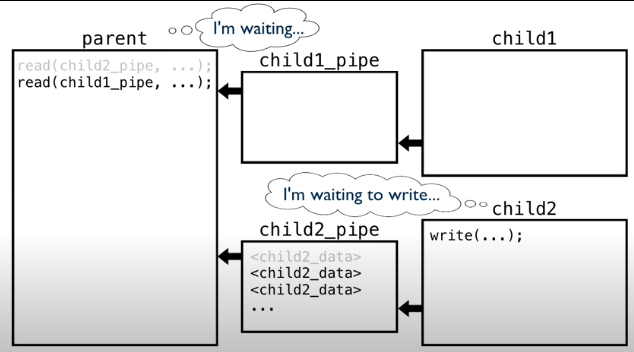
\includegraphics[width=\linewidth]{images/week_10_notes_2_1.png}
        \end{center}
        \item \textit{select} $\leftarrow$ \underline{solution}
        \begin{itemize}
            \item monitors file descriptors, waiting until one or more of the file
            descriptors become ready
        \end{itemize}
    \end{itemize}
\end{itemize}


\bigskip

\section*{Select 2 of 2}

\bigskip

\begin{itemize}
    \item pipe
    \begin{itemize}
        \item is a connection between two processes
        \item is used for passing one process to another
    \end{itemize}

    \begin{lstlisting}[language=c, caption={select\_example\_2\_1.c}]
    #include <stdio.h>
    #include <stdlib.h>
    #include <unistd.h>
    #define MSGSIZE 16
    char* msg1 = "hello, world #1";
    char* msg2 = "hello, world #2";
    char* msg3 = "hello, world #3";

    int main()
    {
        char inbuf[MSGSIZE];
        int p[2], i;

        if (pipe(p) < 0) {
            exit(1);
        }

        /* continued */
        /* write pipe */

        write(p[1], msg1, MSGSIZE); // <- write #1
        write(p[1], msg2, MSGSIZE); // <- write #2
        write(p[1], msg3, MSGSIZE); // <- write #3

        for (i = 0; i < 3; i++) {
            /* read pipe */
            read(p[0], inbuf, MSGSIZE); // <- Read end
            printf("%s\n", inbuf);
        }
        return 0;
    }
    \end{lstlisting}

    \item select
    \begin{itemize}
        \item monitors file descriptors, waiting until one or more of the file
        descriptors become ready
        \item \textbf{Syntax:} int select(numfd, read\_fds, NULL, NULL, NULL);
        \begin{itemize}
            \item \textbf{numfd:} specifies how many descriptors should be examined
            \item \textbf{read\_fds:} points to a bit mask that specifies the file descriptors to check for reading
            \item No need to worry about NULL for now :).
        \end{itemize}
        \item The following macros are used
        \begin{itemize}
            \item \textbf{FD\_SET(\textit{fd}, \textit{\&fdset}):} Sets the bit for the file descriptor \textit{fd} in the file descriptor set \textit{fdset}
            \begin{itemize}
                \item is similar to Python's set
            \end{itemize}
            \item \textbf{FD\_ZERO (\textit{\&fdset}):} Initializes the file descriptor set \textit{fdset} to have zero bits
            \item \textbf{FD\_ISSET(\textit{fd}, \textit{\&fdset}):} Returns a non-zero value if the bit for the file descriptor \textit{fd}
            is set in the file descriptor set pointed by \textit{fdset}, and 0 otherwise
        \end{itemize}
    \end{itemize}


    \begin{lstlisting}[language=c, caption={select\_example\_2\_1.c}]
    #include <stdio.h>
    #include <stdlib.h>
    #include <unistd.h>
    #include <string.h>
    #include <sys/wait.h>

    #define MAXSIZE 4096
    void handle_child1(int *fd);
    void handle_child2(int *fd);

    /* A program to illustrate the basic use of select.
        *
        * The parent forks two children with a pipe to read from each of them and then
        * reads first from child 1 followed by a read from child 2.
    */

    int main() {
        char line[MAXSIZE];
        int pipe_child1[2], pipe_child2[2];

        // Before we fork, create a pipe for child 1
        if (pipe(pipe_child1) == -1) {
            perror("pipe");
        }

        int r = fork();
        // === line below run by parent, child 1 ===
        if (r < 0) {
            perror("fork");
            exit(1);
        } else if (r == 0) {
            handle_child1(pipe_child1);
            exit(0);
        // =========================================
        } else {

            if (pipe(pipe_child2) == -1) {
                perror("pipe");
            }

            r = fork();
            // === line below run by parent, child 2 ===
            if (r < 0) {
                perror("fork");
                exit(1);
            } else if (r == 0) {
                close(pipe_child1[0]);
                handle_child2(pipe_child2);
                exit(0);
            // ======================================
            } else {
                // === line run by parent ===
                close(pipe_child2[1]); // <- pipe closed in parent (since write is for children only)

                // === This part needs to be re-done each time before read by parent===
                fd_set read_fds; // <- creates set
                FD_ZERO(&read_fds); // <- initializes set
                FD_SET(pipe_child1[0], &read_fds); // <- adds
                FD_SET(pipe_child2[0], &read_fds);
                // ==========================

                int numfd;
                if (pipe_child1[0] > pipe_child2[0]) {
                    numfd = pipe_child1[0] + 1;
                } else {
                    numfd = pipe_child2[0] + 1;
                }

                if (select(numfd, &read_fds, NULL, NULL, NULL) == -1) {
                    perror("select");
                    exit(1);
                }

                // Read first from child 1
                if (FD_ISSET(pipe_child1[0], &read_fds)) {
                    if ((r = read(pipe_child1[0], line, MAXSIZE)) < 0) {
                        perror("read");
                    } else if (r == 0) {
                        printf("pipe from child 1 is closed\n");
                    } else {
                        printf("Read %s from child 1\n", line);
                    }
                }

                // Now read from child 2
                if (FD_ISSET(pipe_child2[0], &read_fds)) {
                    if ((r = read(pipe_child2[0], line, MAXSIZE)) < 0) {
                        perror("read");
                    } else if (r == 0) {
                        printf("pipe from child 2 is closed\n");
                    } else {
                        printf("Read %s from child 2\n", line);
                    }
                }
            }
            // could close all the pipes but since program is ending we will just let
            // them be closed automatically
        }
        return 0;
    }

    void handle_child1(int *fd) {
        close(fd[0]);   // close read only part of pipe if children
        printf("[%d] child\n", getpid());
        // Child will write to parent
        char message[10] = "HELLO DAD";
        write(fd[1], message, 10);
        close(fd[1]);
    }

    void handle_child2(int *fd) {
        close(fd[0]);   // close read only part of pipe if children
        printf("[%d] child\n", getpid());
        // Child will write to parent
        char message[10] = "Hi mom";
        write(fd[1], message, 10);
        close(fd[1]);
    }
    \end{lstlisting}


\end{itemize}

\end{document}